%%%%%%%%%%%%%%%%%%%%%%%%%%%%%%%%%%%%%%%%%%%%%%%%%%%%%%%%%%%%%%%%%%%%%%%%%%%%%%%%
%%%%%%%%%%%%%%%%%%%%%%%%%%%%%%%%%%%%%%%%%%%%%%%%%%%%%%%%%%%%%%%%%%%%%%%%%%%%%%%%
%%                                                                            %%
%% thesistemplate.tex version 3.01 (2017/10/06)                               %%
%% The LaTeX template file to be used with the aaltothesis.sty (version 3.01) %%
%% style file.                                                                %%
%%                                                                            %%
%% This is licensed under the terms of the MIT license below.                 %%
%%                                                                            %%
%% Copyright 2017, by Luis R.J. Costa, luis.costa@aalto.fi,                   %%
%% Copyright 2017 documentation in Finnish in the template by Perttu Puska,   %%
%% perttu.puska@aalto.fi                                                      %%
%% Copyright Swedish translations 2014 by Elisabeth Nyberg,                   %%
%% elisabeth.nyberg@aalto.fi and Henrik Wallén, henrik.wallen@aalto.fi        %%
%%                                                                            %%
%% Permission is hereby granted, free of charge, to any person obtaining a    %%
%% copy of this software and associated documentation files (the "Software"), %%
%% to deal in the Software without restriction, including without limitation  %%
%% the rights to use, copy, modify, merge, publish, distribute, sublicense,   %%
%% and/or sell copies of the Software, and to permit persons to whom the      %%
%% Software is furnished to do so, subject to the following conditions:       %%
%% The above copyright notice and this permission notice shall be included in %%
%% all copies or substantial portions of the Software.                        %%
%% THE SOFTWARE IS PROVIDED "AS IS", WITHOUT WARRANTY OF ANY KIND, EXPRESS OR %%
%% IMPLIED, INCLUDING BUT NOT LIMITED TO THE WARRANTIES OF MERCHANTABILITY,   %%
%% FITNESS FOR A PARTICULAR PURPOSE AND NONINFRINGEMENT. IN NO EVENT SHALL    %%
%% THE AUTHORS OR COPYRIGHT HOLDERS BE LIABLE FOR ANY CLAIM, DAMAGES OR OTHER %%
%% LIABILITY, WHETHER IN AN ACTION OF CONTRACT, TORT OR OTHERWISE, ARISING    %%
%% FROM, OUT OF OR IN CONNECTION WITH THE SOFTWARE OR THE USE OR OTHER        %%
%% DEALINGS IN THE SOFTWARE.                                                  %%
%%                                                                            %%
%%                                                                            %%
%%%%%%%%%%%%%%%%%%%%%%%%%%%%%%%%%%%%%%%%%%%%%%%%%%%%%%%%%%%%%%%%%%%%%%%%%%%%%%%%
%%%%%%%%%%%%%%%%%%%%%%%%%%%%%%%%%%%%%%%%%%%%%%%%%%%%%%%%%%%%%%%%%%%%%%%%%%%%%%%%

%\documentclass[english, 12pt, a4paper, elec, utf8, pdfa]{aaltothesis}
\documentclass[english, 12pt, a4paper, elec, utf8, pdfa, online]{aaltothesis}
%\documentclass[english,12pt,a4paper,dvips]{aaltothesis}

\newcommand{\pubdate}{11.5.2018}
%% Use the following options in the \documentclass macro above:
%% your school: arts, biz, chem, elec, eng, sci
%% the character encoding scheme used by your editor: utf8, latin1
%% thesis language: english, finnish, swedish
%% make an archiveable PDF/A compatible file: pdfa
%% symmetric typeset layout and blue hypertext for online publication: online
%%            (no option is the default, resulting in a wide margin on the
%%             binding side of the page and black hypertext)
%% two-sided printing: twoside (default is one-sided printing)
%%

\usepackage{graphicx}
\usepackage{cite}
\usepackage{amsfonts,amssymb,amsbsy}

\usepackage{listings}
\definecolor{commentgreen}{rgb}{0,0.5,0}
\lstset {
    basicstyle=\ttfamily,
    texcl=true,
    tabsize=4,
    keywordstyle=\color{blue},
    commentstyle=\color{commentgreen},
    identifierstyle=\color{black},
    stringstyle=\color{red},
    breaklines=true,
    numbers=left,
    numberstyle={\small \color{black}},
    frame=L,
    %xleftmargint=\parindent,
    framexleftmargin=0.5pt,
    showspaces=false,
    showstringspaces=false
}

\usepackage{chngcntr}
%%\counterwithin{figure}{section}

\degreeprogram{Automation and information technology}
\major{Automation and systems engineering}
\code{AUT}
\univdegree{BSc}

\thesisauthor{Roope Savolainen}
\thesistitle{Modeling and analyzing Helsinki's traffic network using a microscopic simulator}
\place{Espoo}
\date{\pubdate}
\supervisor{Prof.\ Pekka Forsman}
\advisor{Dr Themistoklis Charalambous}

\uselogo{aaltoRed}{''}

\keywords{traffic simulation\spc traffic flow theory\spc fundemental diagram of traffic flow\spc three-phase traffic theory}
\thesisabstract{
	Abstract here.
}

\copyrighttext{Copyright \noexpand\copyright\ \number\year\ \ThesisAuthor}
{Copyright \copyright{} \number\year{} \ThesisAuthor}

\begin{document}

\makecoverpage
\makecopyrightpage

\begin{abstractpage}[english]
	\abstracttext{
    Traffic analysis is the field that studies traffic networks, their behavior and performance. Traffic analysis is an important tool in optimizing and improving society's vital infrastructure. Traffic analysis can be used to identify bottlenecks in a traffic network, find underlying causes for traffic jams and optimize the usage of roads.

    Traffic analysis uses traffic flow models to predict the behavior of traffic networks. Traffic flow models can be roughly divided into two distinct categories; microscopic and macroscopic traffic flow models. In a microscopic model, individial vehicles are modelled using some kinds of behavioral models, whereas in macroscopic models, the traffic is modelled as a whole and described using macroscopic quantities, such as traffic flow and velocity.

    The two traffic flow models discussed in the thesis are the fundemental diagram of traffic flow and the three-phase model of traffic flow. The fundemental diagram approach assumes that the flow rate of traffic can be expressed as a function of traffic density, where the flow rate increases along with the density, until a certain density is hit, after which congestion starts to form and the flow rate begins to diminish. The three-phase model is a refined version of the fundemental diagram approach, where the congestion phase is divided into two phases. First, a synchronized traffic phase forms, which can be thought as an equilibrium between free-flowing traffic and congestion. From that phase, the traffic can transition into a jammed phase, where the velocity of all vehicles drops significantly.

    In this thesis, a microscopically modelled traffic simulation of Helsinki's city centre was created and analyzed. Its behavior was measured and compared to the aforementioned theoretical traffic analysis theories. The results show that that the three-phase model describes the microscopic simulation rather accurately.
    }
\end{abstractpage}

\newpage

\thesistitle{Helsingin liikenneverkon mallintaminen ja analyysi mikroskooppisella simulaatiolla}
\advisor{FT Themistoklis Charalambous}
\degreeprogram{Automaatio- ja informaatioteknologia}
%\department{Elektroniikan ja nanotekniikan laitos}
\major{Automaatio- ja systeemitekniikka}
\keywords{liikennesimulaatio, liikennevirtateoria, liikennevirran perusdiagrammi, kolmivaiheinen liikennemalli}

\begin{abstractpage}[finnish]
    {\scriptsize
    Liikenteen ruuhkautuminen on yhteiskunnalle kallis ilmiö. Jos tieverkosto ei ole riittävän suurelle kulkuneuvomäärälle mitoitettu, sekä kaupallinen, että yksittäisten ihmisten siirtyminen paikasta toiseen on tehotonta. Tieverkon toimivuutta voidaan mitata muun muassa mittaamalla sen virtautta, joka kuvaa sitä, kuinka paljon ajoneuvoja tietyn pisteen läpi ajaa aikayksikössä. Oikeassa maailmassa tapahtuvien mittausten lisäksi tieverkon suorityskykyä voidaan mitata simuloimalla sen toimintaa erilaisissa tilanteissa. Näin on mahdollista tutkia myös esimerkiksi harvinaisempia tai hypoteettia tilanteita.

    Liikennesimulaatiossa käytettävät mallit voidaan karkeasti jakaa kahteen ryhmään, mikrosimulaatioon ja makrosimulaatioon. Mikrosimulaatiossa jokainen ajoneuvo ja sen käyttäytyminen mallinnetaan yksilöllisesti. Makrosimulaatiossa huomiota ei kiinnitetä yksittäiseen ajoneuvoon, vaan liikennevirtaa käsitellään kokonaisuutena, jonka käyttäytyminen muistuttaa esimerkiksi nesteiden virtaamista, jolloin virran etenemistä kuvaillaan suureilla, kuten virtausmäärä tai liikenteen tiheys ja nopeus. Monesti liikennettä tutkittaessa kiinnostuneita ollaan juuri näistä makrotason käyttäytymistä kuvaavista suureista. Näitä suureita voidaan mitata myös mikrotason simulaatiosta tarkastelemalla yksittäisiä pisteitä. Tällöin mielenkiintoiset suureet saadaan tarkasteltaviksi, mutta simulaatiossa voidaan kuitenkin tarkastella yksittäisen ajoneuvon käyttäytymistä.

    Liikenneverkon konkreettinen muokkaaminen on usein hyvin kallis operaatio. Tämän vuoksi liikenteen tehostaminen ilman muutoksia itse tieverkkoon on usein erittäin kustannustehokas tapa purkaa liikenneruuhkia. 

    Kaksi makrotason liikenneanalyysin mallia, joita tässä työssä tarkastellaan, ovat liikennevirran perusdiagrammiin perustuva analyysi, sekä liikenteen kolmivaihemalli. Liikennevirran perusdiagrammiksi kutsutaan kuvaajaa, jossa liikenteen virtausmäärä on esitetty liikennetiheyden funktiona. Perusdiagrammin keskeinen periaate on, että virtausmäärä kasvaa lineaarisesti tiheyden kasvaessa, kunnes saavutetaan tietty, tieosuudelle ominainen tiheys, jonka ohittamisen jälkeen tieosuus alkaa ruuhkautua ja virtausmäärä laskea lineaarisesti.

    Perusdiagrammi on tieteellisen liikenneanalyysin vanhimpia työkaluja, mutta sen heikkoutena voidaan pitää sitä, ettei se kuvaa ruuhkien syntymistä kovinkaan tarkasti, tämän vuoksi on kehitetty uudempia malleja, jotka kuvaavat ruuhkautumista tarkemmin. Yksi näistä on kolmivaiheinen liikennemalli, jossa perusdiagrammin jälkimmäinen osa on jaettu kahteen osaan, niin sanottuun synkronoidun liikenteen osaan ja ruuhkaosaan. Tämä malli vastaa todellista liikennettä perusdiagrammia tarkemmin.

    Tässä työssä tutkittiin Helsingin keskusta-alueen liikenneverkkoa simuloimalla sen toimintaa Vissim-liikennesimulaatio-ohjelmiston avulla. Vissim mallintaa liikenteen mikrosimulaatio-mallilla, joten yksittäisten autojen käyttäytymistä voidaan tutkia ja ohjata ohjelmallisesti. Simulaatiosta kerättiin makrotason mittausdataa, jonka pohjalta liikenneverkon käyttäytymistä voitiin analysoida käyttämällä edellämainittuja makrotason malleja. Työssä tarkasteltiin, kuinka mallit suoriutuvat mikrotason simulaation tulosten ennustamisesta. Kun simulaatio suoritettiin ja sen käyttäytiminen analysoitiin, todettiin kolmivaiheisen liikennemallin kuvaavan lopputuloksia hyvällä tarkkuudella.
    }

\end{abstractpage}

\newpage

%% Preface
%%
%%\mysection{Preface}
%\mysection{Esipuhe}
%%I want to thank Professor Pirjo Professori and my instructor Dr Alan Advisor for
%%their good and poor guidance.\\

%%\vspace{5cm}
%%Otaniemi, \pubdate

%%\vspace{5mm}
%%{\hfill Roope A.\ Savolainen \hspace{1cm}}

%% Force a new page after the preface
%%
%%\newpage


\thesistableofcontents

\cleardoublepage

\section{Introduction}

\thispagestyle{empty}

Traffic jams are not only an annoyance in our everyday lives, but also a burden on the efficient functioning of the society. One of the basic tasks of a state is to build and maintain infrastructure that is sufficient to support the local economy, but the rapidly developing urban areas do not make it an easy one.

This thesis will examine Helsinki's traffic network. The city centre of Helsinki was originally built in the 19th century, but the population of the city has grown over ten-fold since then \cite{helsinki}. To cope with the resulting dramatic increase in traffic amounts traffic control methods are usually implemented instead of building new infrastructure. For example, congestion pricing models have been implemented in cities such as London and Stockholm to protect areas most susceptible to congestion \cite{congestionpricing}.

Traffic flow research attempts to model the behavior of real-life traffic networks. Theoretical, empirically verified models of traffic can be useful in comparing traffic control methods and determining optimal ways to control traffic and minimize congestion.

The goal of this thesis is to simulate Helsinki's traffic network using Vissim traffic simulation software and analyze its behavior using traffic flow theories. The thesis is divided into five sections. In section \ref{bg}, the theoretical basis behind the used traffic simulation methods will be explored. The simulation methods and used material will be described in section \ref{experiment}. The results of the simulation will be presented in section \ref{res}. Analysis of the results will be conducted in section \ref{discussion}.

\clearpage

\section{Background} \label{bg}

\subsection{Microscopic and macroscopic simulation}

The field of traffic flow examines vehicle traffic on road networks. There are several different models used in analyzing traffic flow. This thesis uses the microscopic and macroscopic models. The microscopic model is used to model the traffic in the developed simulation and values describing the macroscopic model will be derived from the simulation.

Microscopic traffic flow modelling simulates the behavior of each individual vehicle. Two common approaches to microsimulation are the car-following models and the cellular automata based models. The car-following approach models the behavior of vehicles in such a way that they try to keep a time distance to the vehicle in front of them. On top of this, the models based on car-following can specify the acceleration behavior, braking strategy and other more sophisticated properties of the modelled vehicles. In cellular automata models, the road is divided into cells and the vehicles move between the cells in discrete steps. Compared to car-following models, cellular automata models tend to be considerably simpler and faster to execute. However, since cellular automata approaches are grid based, measurements from them are not as realistic as ones from car-following simulations.

As opposed to microscopic models, macroscopic traffic flow models do not consider individual vehicles, but model the vehicle flow similarly to liquids and gases. The important quantities of traffic in this model are the flow density $\rho$, flow rate $Q$ and vehicle velocity $v$. The quantities are related by the flow-density relation

\[ Q = \rho v .\]

As the macroscopic quantities are useful in analyzing a traffic network, it is important that they can be measured in a microscopic simulation. Flow rate can be measured from a microscopic model by counting the number of vehicles passing a point on a road. Also the velocity of vehicles is explicitly modeled in microscopic simulation models, so it is also possible to get the average velocity of a group of vehicles. Based on the flow rate and velocity we can also calculate the density of the traffic in the model. \cite{treiber}

\subsection{Fundemental diagram of traffic flow}

There are a number of macroscopic theories attempting to explain the behavior of traffic. A widely-used approach is the fundemental diagram of traffic flow. In these models traffic flow is considered a function of traffic density. The diagram is triangular and the maximum value of flow rate is at density $\rho_c$, which is called the critical density. Before reaching the critical density, the flow rate increases with the density. After the traffic passes the critical density, congestion starts to form and the flow rate declines. Hence, under the fundemental diagram based approaches, traffic is divided into two distrinct phases, free-flowing and congested, depending on the traffic density. \cite {lighthillwhitham}

\begin{figure}[h]
    \centering
    \includegraphics[width=0.75\textwidth]{graphs/fund_diagram}
    \caption{The fundemental diagram of traffic flow}
\end{figure}

\subsection{Three-phase model}

Another model to explain real-life traffic dynamics is the three-phase traffic theory. Unlike the fundemental diagram approach, which divided traffic into two phases, the three-phase model introduces two new phases, synchronized flow and wide moving jam, that replace the congested phase of the earlier theories. Therefore, the three-phase model includes a total of three traffic phases, the free-flowing, the synchronized flow and the moving jam.

Free-flowing traffic refers is used similarly as in fundemental diagram based approaches. It is the phase when an increase in traffic density will not cause congestion. Synchronized flow refers to a state where the traffic flow is mostly continuous and there are few stops. Also in synchronized flow, the traffic limits the velocities of all vehicles to a certain value, so the velocities tend to be locally synchronized. The wide moving jam phase is a state, where all the vehicles in the jam have the same mean velocity and where the mean velocity persists through possible traffic bottlenecks. These phases are referred to as F (free-flowing), S (synchronized flow) and J (wide moving jam) in some contexts in this thesis.

The phase transition F $\to$ S always occurs, when the traffic density exceeds $\rho_c$. This can be caused by bottlenecks, such as changes in the number of available lanes. If the traffic density, however is close to $\rho_c$, but still under it, an F $\to$ S transition can also be caused by random local disturbances of the traffic, such as a driver braking in free-flowing traffic. These probability of these local disturbances causing the transition is higher near the critical density. Because traffic can transition to the synchronized flow phase even before the critical density, the flow rate in the synchronized flow phase cannot be represented as a funtion of flow density.

Instead of a line, an area can be drawn in the flow-density diagram, where possible points in the synchronized flow phase lie. The upper bound of the area describes the largest flow rate that a density can support. This line is the situation where drivers keep the lowest safety gap that they can. The lower edge is a state where the time gaps between the vehicles in traffic grow so large that the driver decides to accelerate and close the gap.

\begin{figure}[h]
    \centering
    \includegraphics[width=0.75\textwidth]{graphs/3phase_fs_diagram}
    \caption{The flow-density diagram in a three-phase model. The line F shows the flow-rates in the free-flowing phase as a function of traffic density. The area S shows potential flow-density points in the synchronized flow phase. }
\end{figure}

The transition S $\to$ J is usually caused by disturbances of traffic, while in the S phase. This can cause the traffic to jam and the vehicle flow to slow down significantly. This is easy to see by examining a time series of vehicle velocity. \cite{kerner}

\begin{figure}[h]
    \centering
    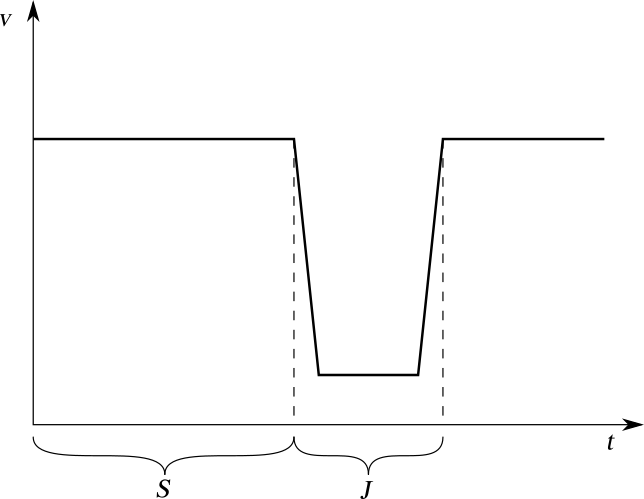
\includegraphics[width=0.75\textwidth]{graphs/3phase_vt}
    \caption{The time series of vehicle velocities in a traffic system, where the traffic temporarily becomes jammed, according to the three-phase model. $S$ and $J$ phases are notated. }
\end{figure}

\clearpage

\section{Research material and methods} \label{experiment}

In this thesis, a microsimulation of the Helsinki city centre area was carried out. The simulation was developed using the microsimulation software PTV Vissim. The goal of the simulation was to examine the capacity and perfomance of the road network in Helsinki's city centre. After running the simulation with varying parameters, its behavior was analyzed using the macroscopic frameworks outlined in the background section.

\subsection{Map data}

The first step in developing the simulation was creating the road network for the simulation. The simulated area is relatively large, but not large enough for modelling the roads by hand to be an unreasonably large task. However, map data of the desired area was available from OpenStreetMap, under the Open Database License. \cite{osm}

After downloading the data, it was roughly cropped to the desired area and converted into a file format compatible with PTV Vissim, with another software, PTV Visum. Once the map data could be imported to Vissim, additional manual adjustments were made so that the simulation would work smoothly. These adjustments included removing small road sections that would not be used during the simulation and remaking some turns that were previously too sharp for the simulated vehicles to take.

\begin{figure}[h]
    \centering
    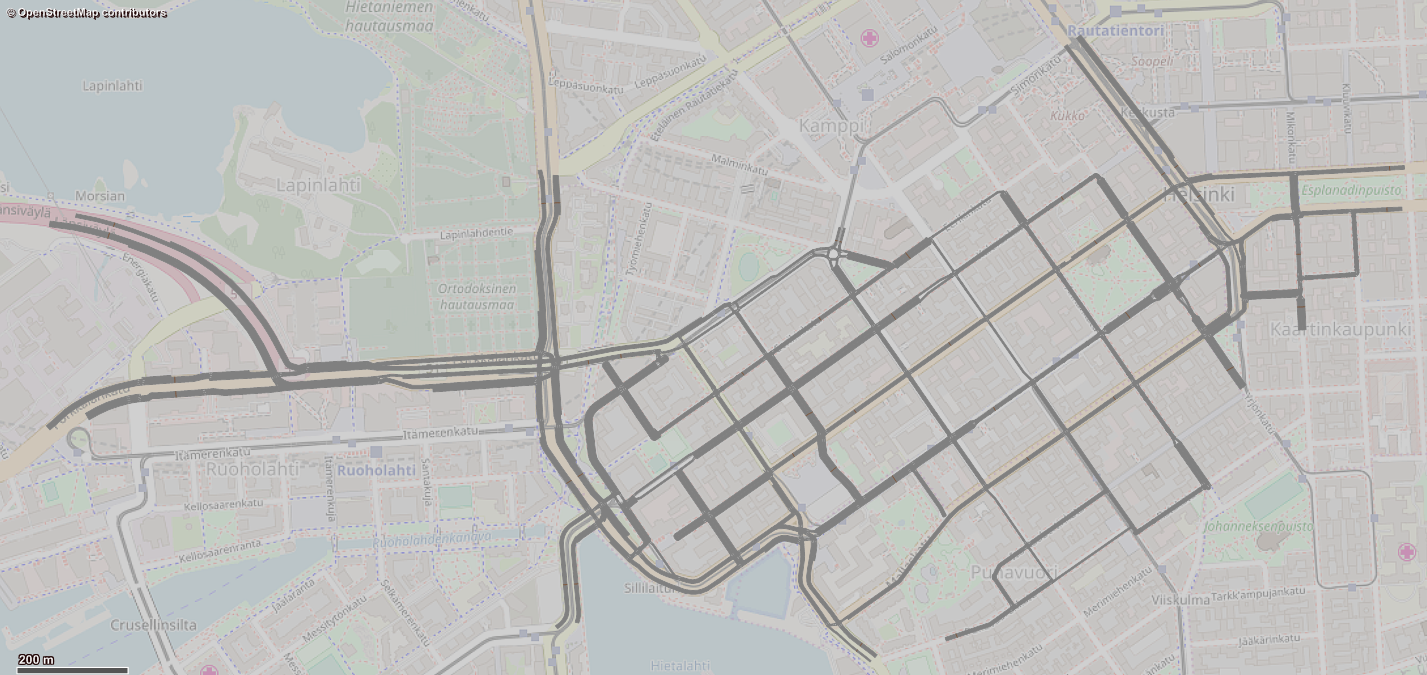
\includegraphics[width=0.9\textwidth]{graphs/vissim_map}
    \caption{The simulation area. Simulation roads shown with dark gray. Background map by OpenStreetMap\cite{osm}.}
\end{figure}

\subsection{Traffic}

After the map data was prepared, traffic inputs and sinks were defined for the simulation. Several entry and exit points for vehicles were placed at roads that enter or leave the simulation area. The dynamic traffic assignment in Vissim models traffic by using traffic demand data for the entry and exit points of the network. In the simulation, traffic demand data was supplied using a demand matrix (i.e. a matrix with $n$ columns and $m$ rows, where $n$ is the number of exit points, $m$ is the number of entry points and the column $i$ on the row $j$ is the flow rate from entry point $j$ to exit point $i$).

At first, these flow rates were simply estimated. However, the realism of the simulation is greatly dependant on having realistic traffic data and the validity of measurements based on this sort of data would be dubious. The demand values were refined with real-life road usage data from the area, published by the Helsinki Urban Environment Division \cite{trafficamounts}. Data for the biggets roads that were assigned as entry or exit points could be found in the dataset, but some had to be estimated. Traffic amounts between 8:00 and 9:00 were chosen, therefore the simulation should represent the morning commute period.

This approach of modelling traffic amounts was chosen because it was easy to implement and iterate on during the development of the simulation. However, it can also bring inaccuracies to the simulation. In the simulation, all traffic runs through the simulated traffic network due to the nature of the traffic demand modelling, but this is not the case in reality. In the real environment we're simulating, there is also traffic inside the simulation area, that this simulation fails to account for. Examining the effects of these inaccuracies and developing a more accurate simulation could be subjects for further work.

\begin{figure}[h]
    \centering
    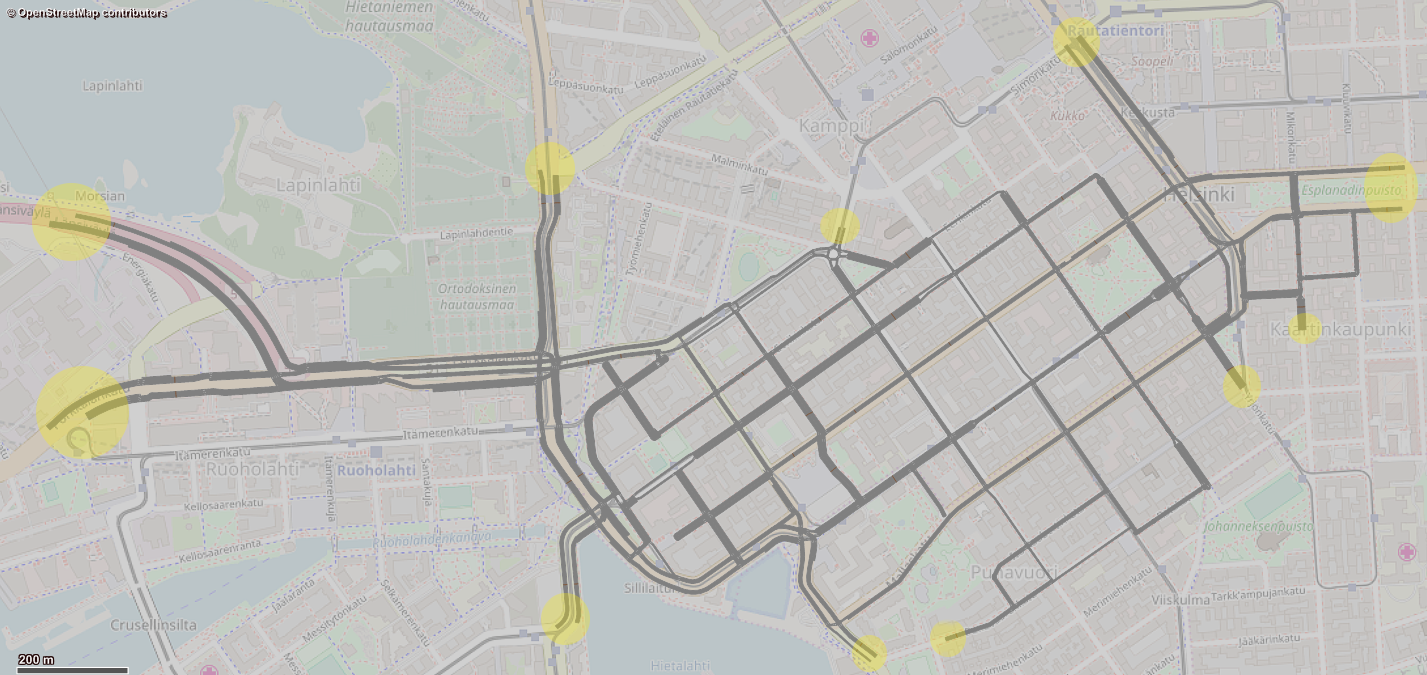
\includegraphics[width=0.9\textwidth]{graphs/vissim_map_entries}
    \caption{The simulation area. Exit and entry points highlighted with yellow. Background map by OpenStreetMap\cite{osm}.}
\end{figure}

\subsection{Data collection} \label{data}

To analyze the macroscopic behavior of the simulation, the flow rate and the velocity of traffic should be measured from the simulation, as mentioned in the background section. Vissim features data collection points that can be placed on the and that automatically record the flow rate and the average velocity of traffic for the point in time periods of configurable length. Data collection points were placed several points in the simulation network. 

After running the simulation, data for flow rate and average velocity could be measured for each measurement period. Based on the flow rate and velocity, traffic density could be calculated. Based on these quantities, an analysis of the network could be carried out.

\subsection{Running the simulation}

Once developed, the simulation was executed repeatedly. Each of the simulation runs was 30 minutes long in simulation time. In order to gather a comprehensive set of data on the traffic network usage, the traffic demand was adjusted between the runs by defining a factor for each run and multiplying all values of the traffic demand matrix by the factor. 6 different values ranging from $0.5$ to $2.5$ were used for different runs A full data set, as described in section \ref{data}, was collected for all runs. After data for the simulation runs was collected, it was used to analyze the traffic at the set data collection points. Velocity time series plots were drawn for all different traffic demand amounts. Also flow-density and velocity-density diagrams were drawn for all data measurement points, aggregating data from all the runs with differing traffic demands.

Vissim's Component Object Model (COM) interface was used to run the simulation. The COM interface is an inter-process communication method that allows for programmatic manipulation of the traffic network and automated usage of the software. The Python programming language and its pywin32 library were used to interface with Vissim via the COM interface to automate varying the traffic demand amounts and running the simulation. Collecting traffic data from Vissim was also done via the Python code and the collected data was used to draw the aforementioned diagrams the Python library matplotlib. All used code can be found in Appendix \ref{code}.

\clearpage

\section{Results} \label{res}

After running the developed simulation and collecting traffic data, diagrams were examined to find points of interest in the traffic network. Points of particular interest would be points were the traffic gets jammed as the traffic flow increases. Diagrams \ref{fig:1} through \ref{fig:4} show selected data collection points that are going to be examined in section \ref{discussion}. These measurements were selected on the basis that they visualize the phenomena described in section \ref{bg}. Many of the measurement points also produced results similar to the ones pictured here, so they aren't separately discussed.

Appendix \ref{graphs} contains flow-density and speed time series graphs for all used data collection points.

\begin{figure}[ht!]
    \centering
    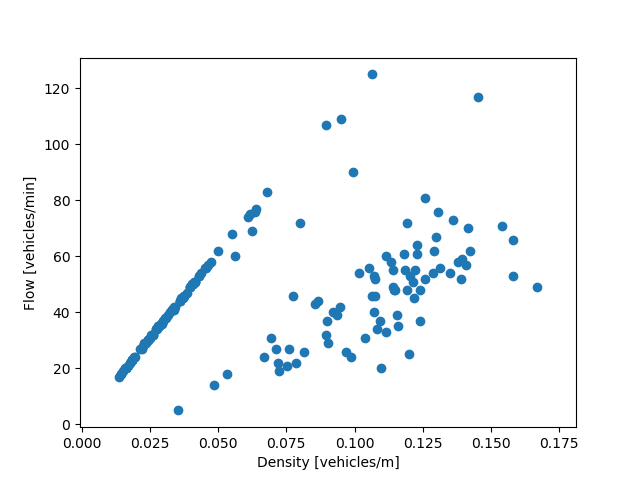
\includegraphics[width=0.9\textwidth]{graphs/Lansivayla_2_flw_dns.png}
    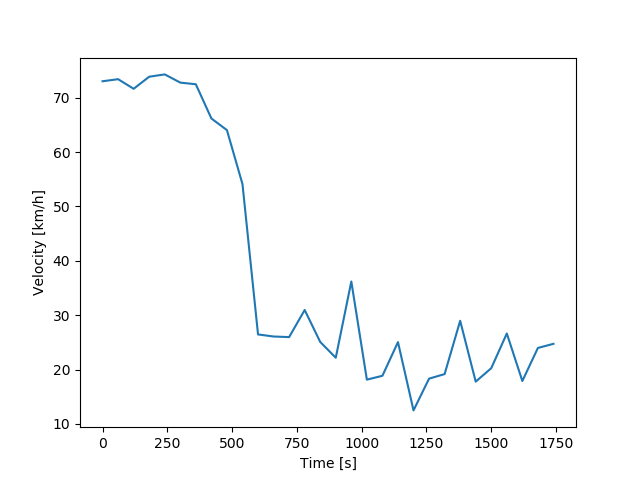
\includegraphics[width=0.9\textwidth]{graphs/Lansivayla_2_spd_time_4.png}
    \caption{Flow-density and velocity time series diagrams for Länsiväylä, measurement point 2.}
    \label{fig:1}
\end{figure}

\begin{figure}[ht!]
    \centering
    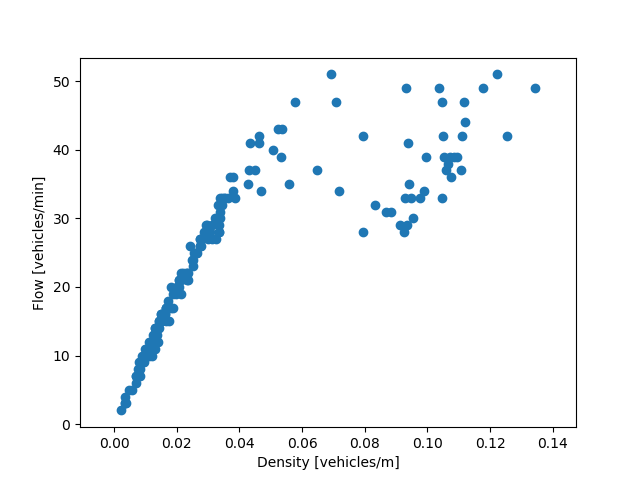
\includegraphics[width=0.9\textwidth]{graphs/Mechelininkatu_1_flw_dns.png}
    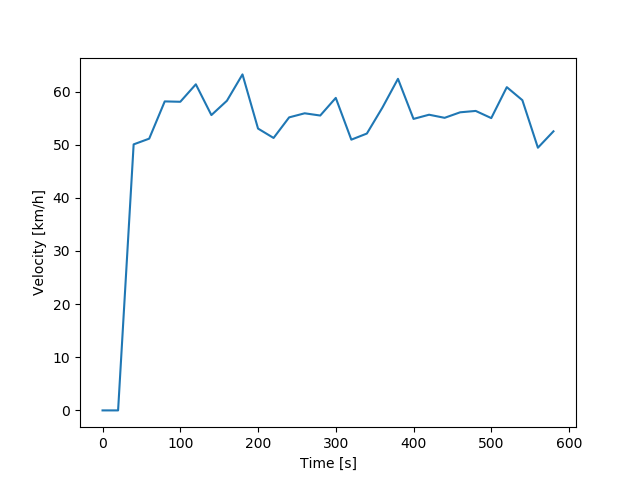
\includegraphics[width=0.9\textwidth]{graphs/Mechelininkatu_1_spd_time_5.png}
    \caption{Flow-density and velocity time series diagrams for Mechelininkatu, measurement point 1.}
    \label{fig:2}
\end{figure}

\begin{figure}[ht!]
    \centering
    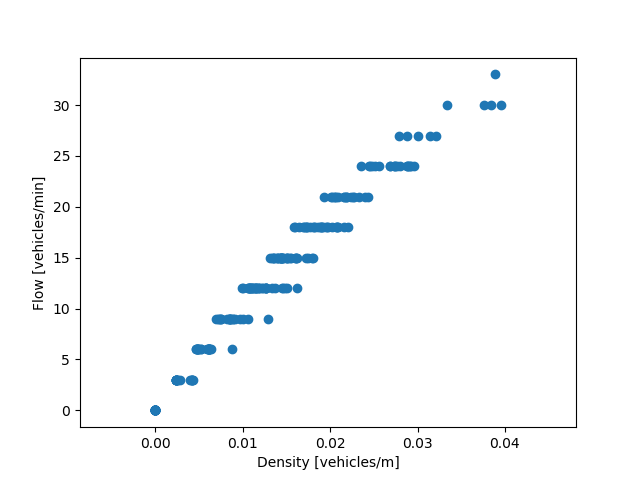
\includegraphics[width=0.9\textwidth]{graphs/Mechelininkatu_4_flw_dns.png}
    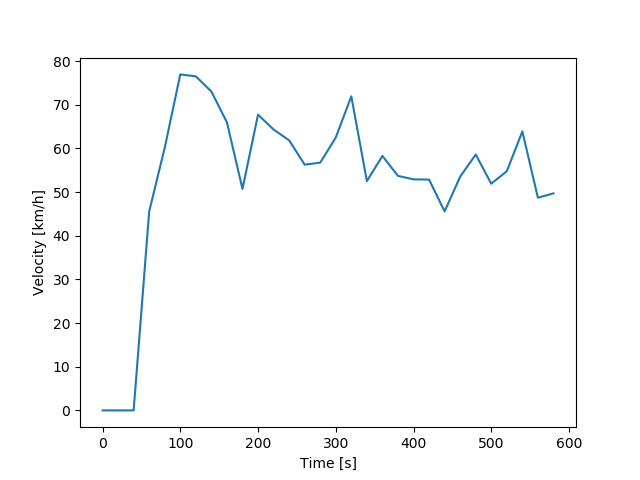
\includegraphics[width=0.9\textwidth]{graphs/Mechelininkatu_4_spd_time_6.png}
    \caption{Flow-density and velocity time series diagrams for Mechelininkatu, measurement point 4. The velocity time series is for the highest simulated traffic demand.}
    \label{fig:3}
\end{figure}

\begin{figure}[ht!]
    \centering
    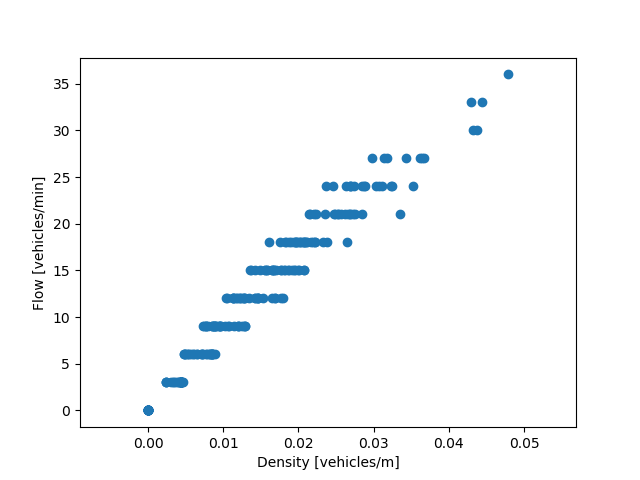
\includegraphics[width=0.9\textwidth]{graphs/Uudenmaankatu_2_flw_dns.png}
    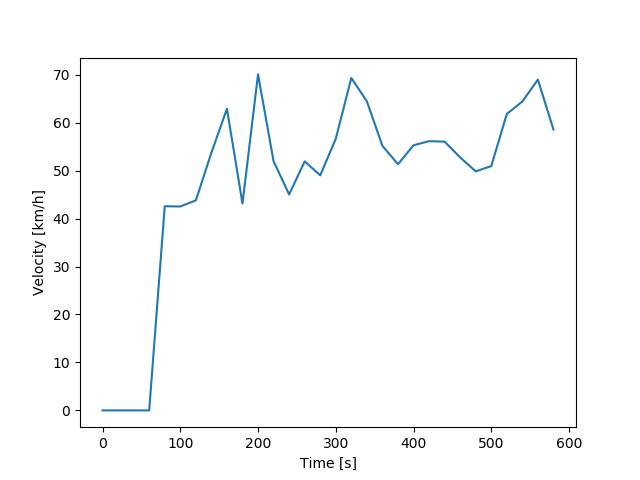
\includegraphics[width=0.45\textwidth]{graphs/Uudenmaankatu_2_spd_time_4.png}
    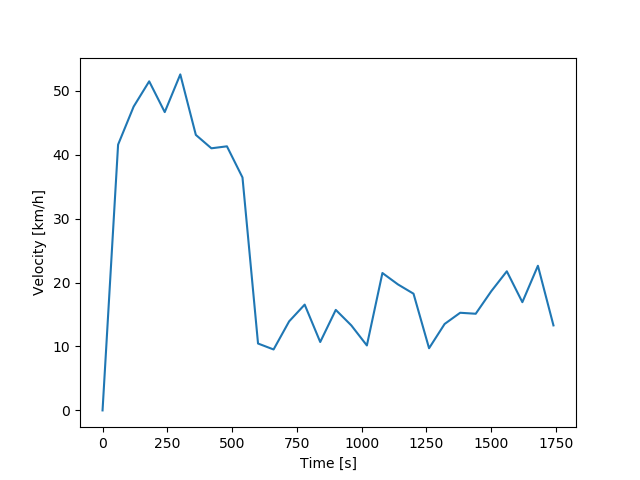
\includegraphics[width=0.45\textwidth]{graphs/Uudenmaankatu_2_spd_time_5.png}
    \caption{Flow-density and two velocity time series diagrams for Uudenmaankatu, measurement point 2. The velocity time series diagram on the left is for a lower traffic demand simulation run than the one on the right.}
    \label{fig:4}
\end{figure}

\clearpage

\section{Discussion} \label{discussion}

In this chapter, the selected results introduced in section \ref{res} will be examined. The descriptiveness of the theories described in section \ref{bg}, in particular the three-phase model, will be analyzed.

Traffic data of Länsiväylä is pictured in figure \ref{fig:1}. From the flow-density diagram, we can see that at first, as the density of vehicles grows, the flow rate also grows along linearly. However as the density surpasses approximately $0.05 vehicles/m$, the flow rate stops reliably growing along with the density. Instead the flow rates roughlt fall inside an area between the $x$-axis and the linear curve that flow and density seem to follow at first. This seems to correspond with the three-phase traffic model and show the $F \to S$ transition of the traffic. The same kind of a shape can also be seen in the flow-density diagrams in figures \ref{fig:2} and \ref{fig:4}.

If the velocity time series data of Länsiväylä is examined, a clear drop in velocity can be seen at around $500$ seconds. This seems to mark the point in which traffic shifts from phase $S$ to $J$, according to the three-phase model. In the case of Länsiväylä, the $J$ phase persists until the end of the simulation round. In contrast to this, the velocity time series of Mechelininkatu (measurement point 1), pictured in figure \ref{fig:2}, drops similarly. However, in the latter case, the velocity gradually recovers to its original value. This demonstrates that a traffic system can recover from a jam without active measures and with a constant traffic demand.

Figure \ref{fig:3} shows a different measurement point of Mechelininkatu, which is located further from the bottleneck areas that the one pictured in figure \ref{fig:2}. As can be seen from the flow-density diagram, the spot does not reach a sufficient traffic density to shift into the $S$ phase of the three-phase model. This is also visible in the velocity time series, which shows a nearly constant velocity throughout the simulation. As can be seen by examining the full dataset in appendix \ref{graphs}, similarly a large portion of data collection points did not exhibit signs of getting jammed. The bottlenecks of the simulation were located around a handful of critical points of the road network.

In figure \ref{fig:4}, the flow-density diagram is drawn along with two velocity time series graphs for two different traffic demand values for a measurement point in Uudenmaankatu. The simulation run with the smaller traffic demand value does show signs of a jam, but as the amount of vehicles entering the simulation is increased with the larger traffic demand, a jam forms in the run with the larger demand. In the pictured data this can be seen as a noticeable velocity drop, indicating a shift into the $J$ phase in the latter graph. This suggests that the increase in traffic density between the runs passes the critical density $\rho_c$, shifting the traffic into phase $S$ and making $S \to J$ transitions possible.

After looking at the major types of measurement results, the three-phase model of traffic seems to explain the different observed phenomena with sufficient accuracy. In comparison to the fundemental model of traffic flow, it provides a more detailed model of how congestion forms in a traffic network. Moreover, its predictions match well with the results derived from the microscopic simulation developed here, while the simplistic near-linear drop after passing $\rho_c$, described by the fundemental diagram does not match the data from the simulation.

Conducting an in-depth discussion on mitigating the bottlenecks in a traffic network is out of scope for this thesis. However, it can be mentioned that congestion pricing has been is seen as an efficient method of reducing congestion in critical roads. Congestion pricing would incentivize both temporal and geographic decentralization of traffic, thus alleviating the worst bottlenecks during peak hours. \cite{congestionpricing}

\clearpage

\thesisbibliography

\bibliography{bibliography}{}
\bibliographystyle{ieeetr}

\clearpage

\thesisappendix

\section{Python code} \label{code}

Below is the Python code used to run the simulation and collect data. Running the code requires the Python libraries matplotlib and pywin32. The code is run by simply running \begin{verbatim}python main.py\end{verbatim}

\begin{verbatim}main.py\end{verbatim}
\lstinputlisting[language=Python]{code/main.py}

\begin{verbatim}simulation.py\end{verbatim}
\lstinputlisting[language=Python]{code/simulation.py}

\begin{verbatim}datacollector.py\end{verbatim}
\lstinputlisting[language=Python]{code/datacollector.py}

\begin{verbatim}figure.py\end{verbatim}
\lstinputlisting[language=Python]{code/figure.py}

\begin{verbatim}settings.py\end{verbatim}
\lstinputlisting[language=Python]{code/settings.py}

\clearpage

\section{Data} \label{graphs}

Flow-density and time series diagrams are presented here for all the data collection points of the simulation. For time series diagrams, only the run with the highest traffic demand will be presented in the interest of conciseness.

It is worth noting that in some velocity graphs quick spikes to zero and back can be seen. This is caused by the low utilization of some of the road segments, and therefore a sign of no traffic passing through the measurement point, instead of a dramatic slowdown of traffic.

\clearpage
\begin{figure}[ht!]
    \centering
    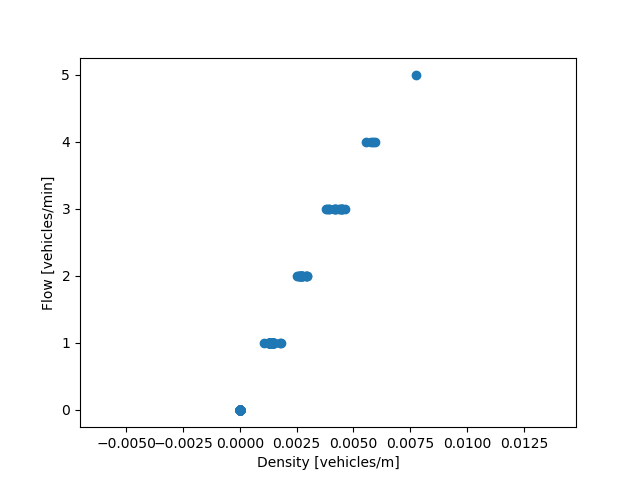
\includegraphics[width=0.45\textwidth]{graphs/Abrahamintie_1_flw_dns.png}
    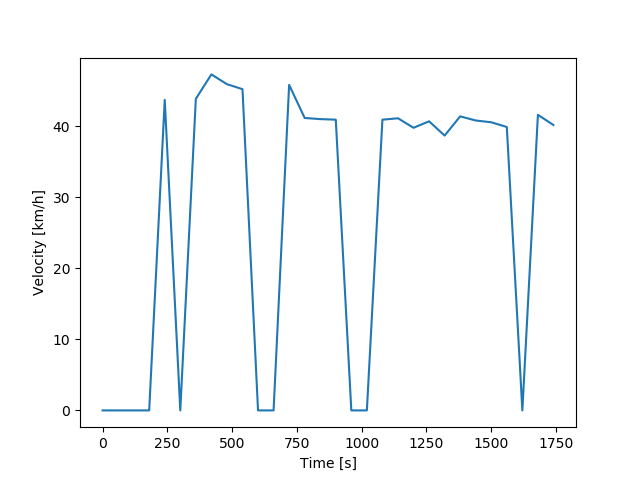
\includegraphics[width=0.45\textwidth]{graphs/Abrahamintie_1_spd_time_6.png}
    \caption{Flow-density and velocity time series diagrams for Abrahamintie, measurement point 1.}
\end{figure}
\begin{figure}[ht!]
    \centering
    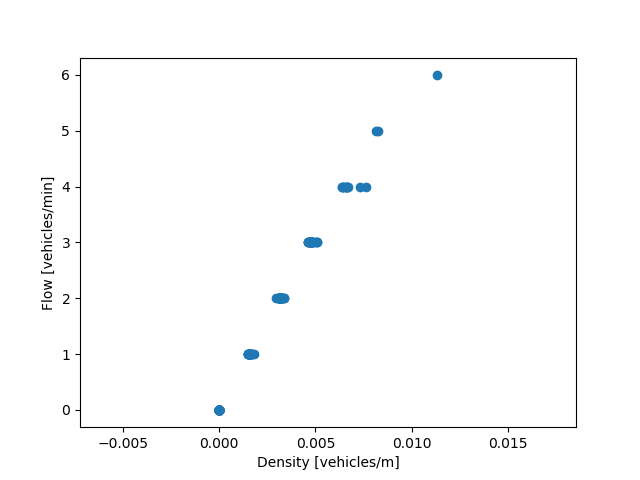
\includegraphics[width=0.45\textwidth]{graphs/Abrahamintie_2_flw_dns.png}
    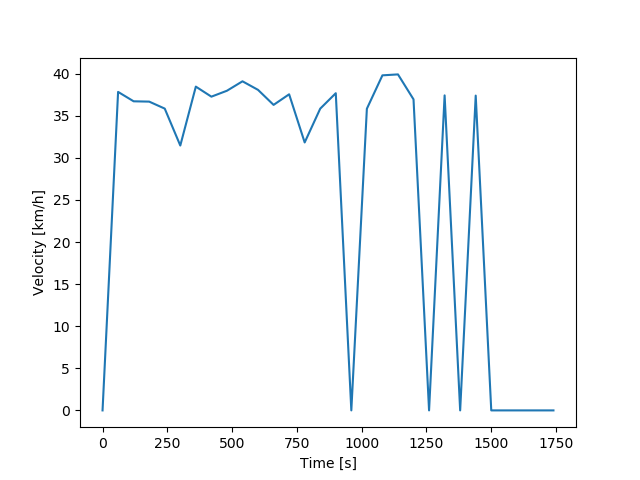
\includegraphics[width=0.45\textwidth]{graphs/Abrahamintie_2_spd_time_6.png}
    \caption{Flow-density and velocity time series diagrams for Abrahamintie, measurement point 2.}
\end{figure}
\begin{figure}[ht!]
    \centering
    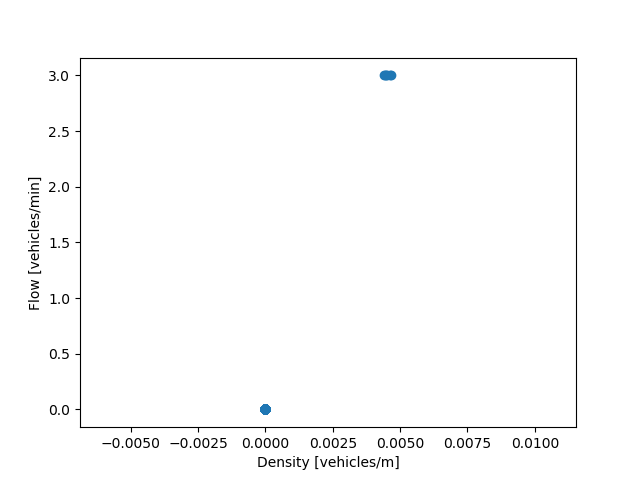
\includegraphics[width=0.45\textwidth]{graphs/Abrahamintie_3_flw_dns.png}
    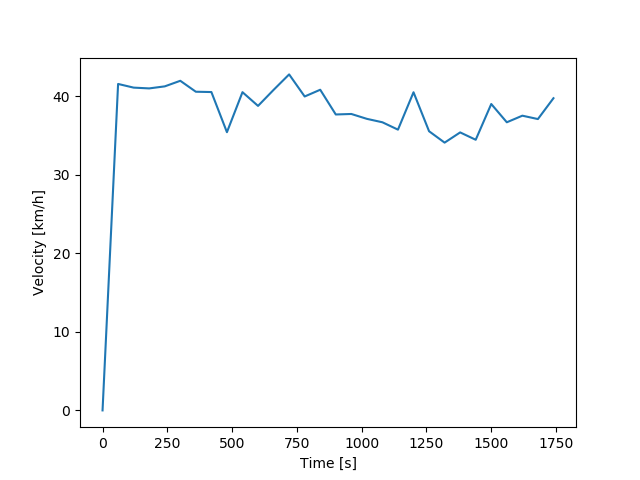
\includegraphics[width=0.45\textwidth]{graphs/Abrahamintie_3_spd_time_6.png}
    \caption{Flow-density and velocity time series diagrams for Abrahamintie, measurement point 3.}
\end{figure}

\clearpage
\begin{figure}[ht!]
    \centering
    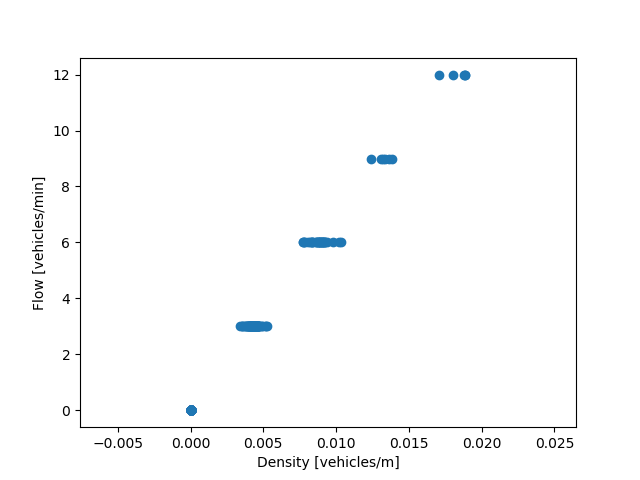
\includegraphics[width=0.45\textwidth]{graphs/Abrahamintie_4_flw_dns.png}
    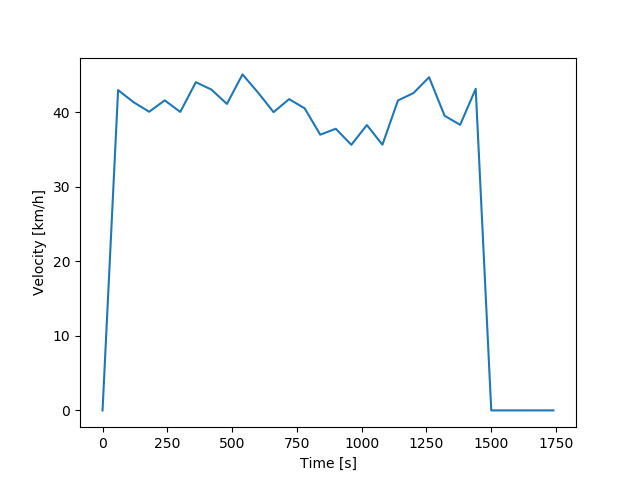
\includegraphics[width=0.45\textwidth]{graphs/Abrahamintie_4_spd_time_6.png}
    \caption{Flow-density and velocity time series diagrams for Abrahamintie, measurement point 4.}
\end{figure}
\begin{figure}[ht!]
    \centering
    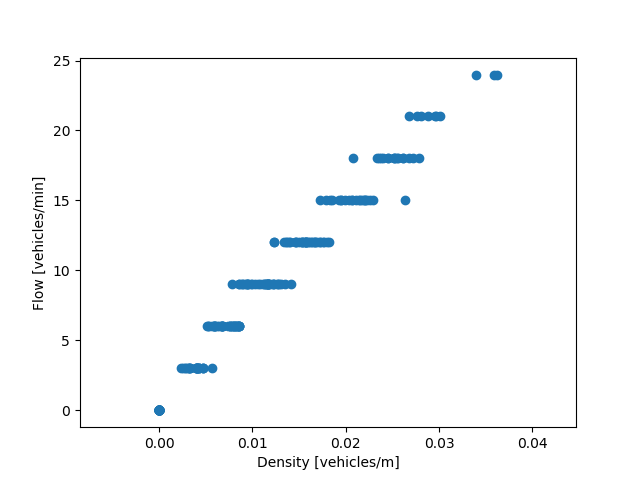
\includegraphics[width=0.45\textwidth]{graphs/Bulevardi_1_flw_dns.png}
    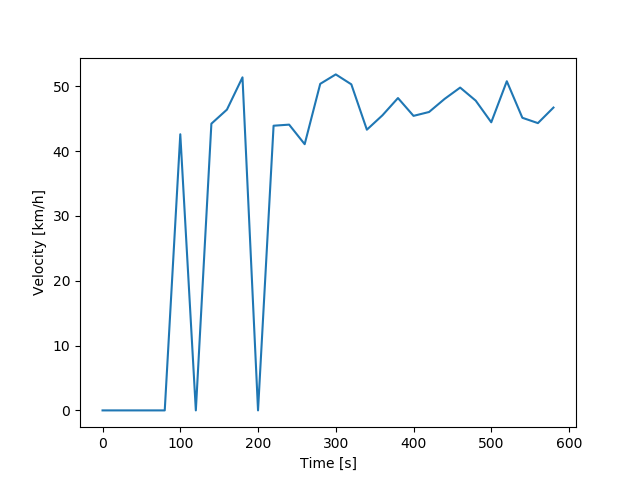
\includegraphics[width=0.45\textwidth]{graphs/Bulevardi_1_spd_time_6.png}
    \caption{Flow-density and velocity time series diagrams for Bulevardi, measurement point 1.}
\end{figure}
\begin{figure}[ht!]
    \centering
    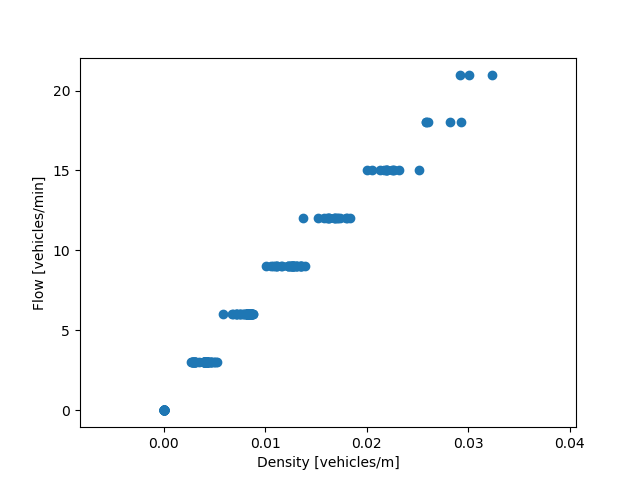
\includegraphics[width=0.45\textwidth]{graphs/Bulevardi_2_flw_dns.png}
    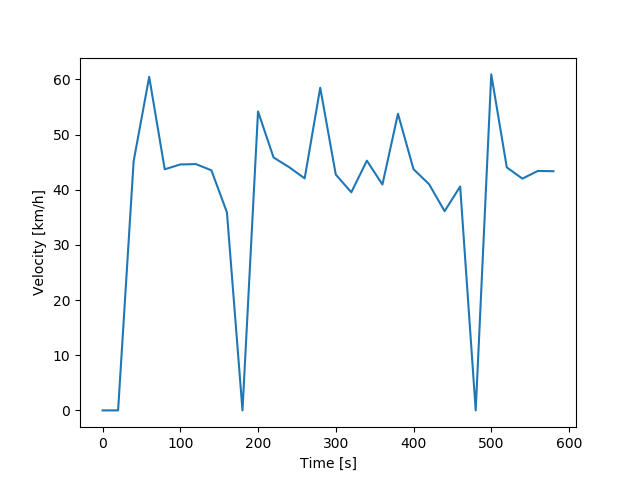
\includegraphics[width=0.45\textwidth]{graphs/Bulevardi_2_spd_time_6.png}
    \caption{Flow-density and velocity time series diagrams for Bulevardi, measurement point 2.}
\end{figure}

\clearpage
\begin{figure}[ht!]
    \centering
    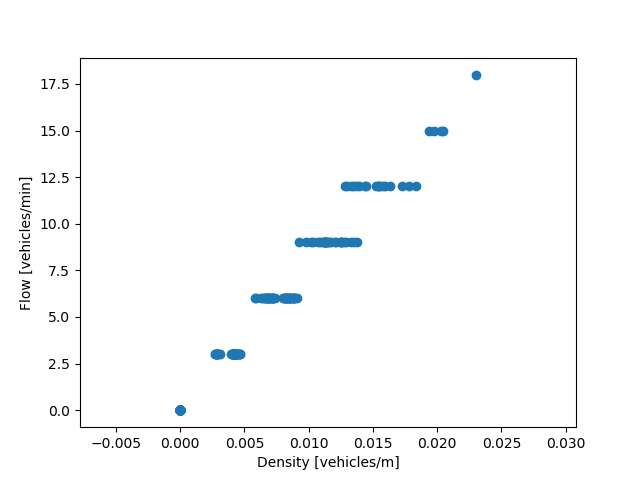
\includegraphics[width=0.45\textwidth]{graphs/Bulevardi_3_flw_dns.png}
    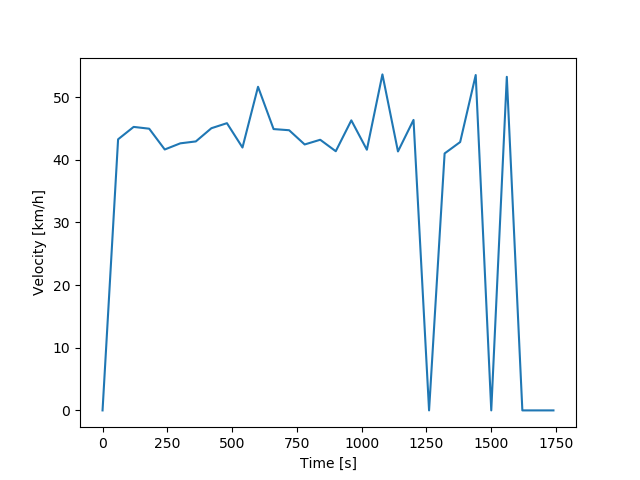
\includegraphics[width=0.45\textwidth]{graphs/Bulevardi_3_spd_time_6.png}
    \caption{Flow-density and velocity time series diagrams for Bulevardi, measurement point 3.}
\end{figure}
\begin{figure}[ht!]
    \centering
    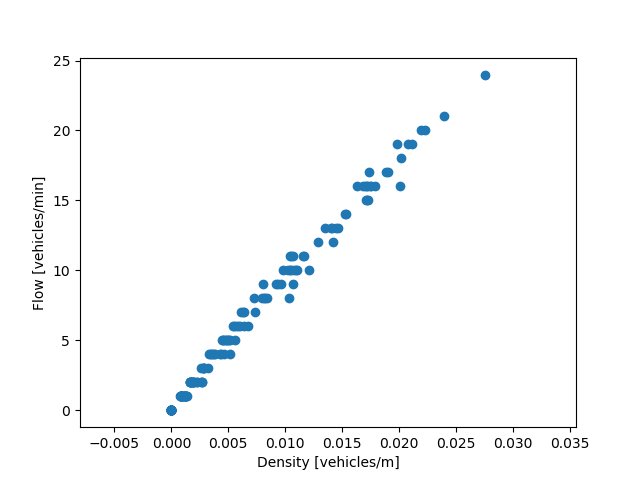
\includegraphics[width=0.45\textwidth]{graphs/Bulevardi_4_flw_dns.png}
    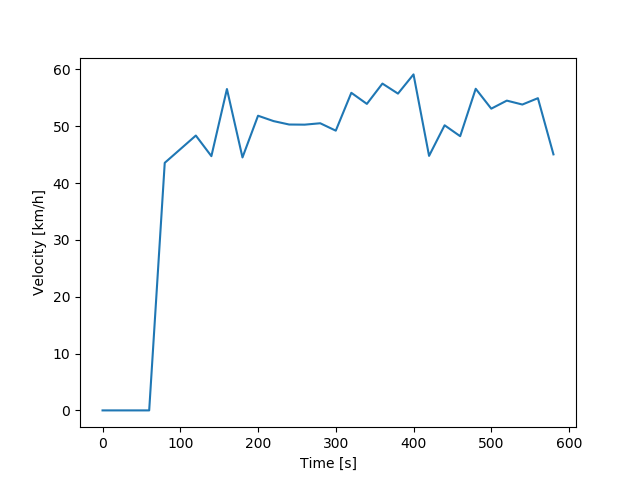
\includegraphics[width=0.45\textwidth]{graphs/Bulevardi_4_spd_time_6.png}
    \caption{Flow-density and velocity time series diagrams for Bulevardi, measurement point 4.}
\end{figure}
\begin{figure}[ht!]
    \centering
    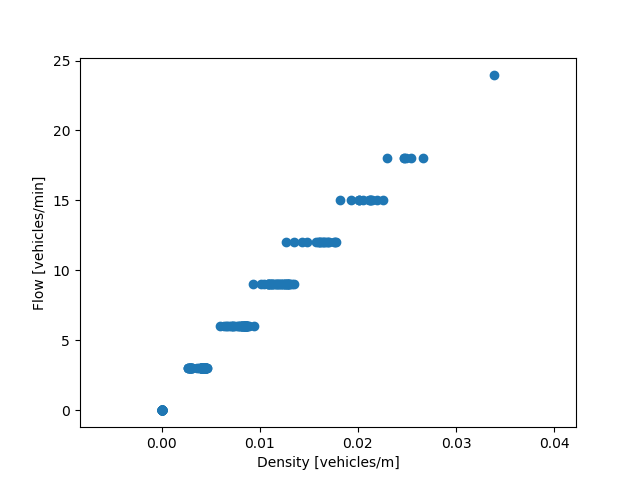
\includegraphics[width=0.45\textwidth]{graphs/Bulevardi_5_flw_dns.png}
    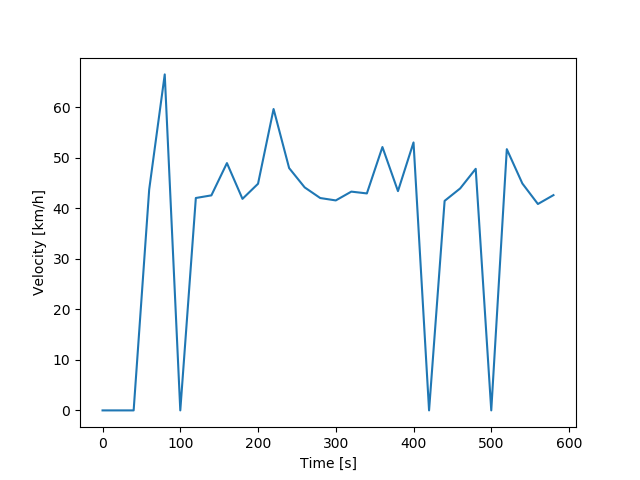
\includegraphics[width=0.45\textwidth]{graphs/Bulevardi_5_spd_time_6.png}
    \caption{Flow-density and velocity time series diagrams for Bulevardi, measurement point 5.}
\end{figure}

\clearpage
\begin{figure}[ht!]
    \centering
    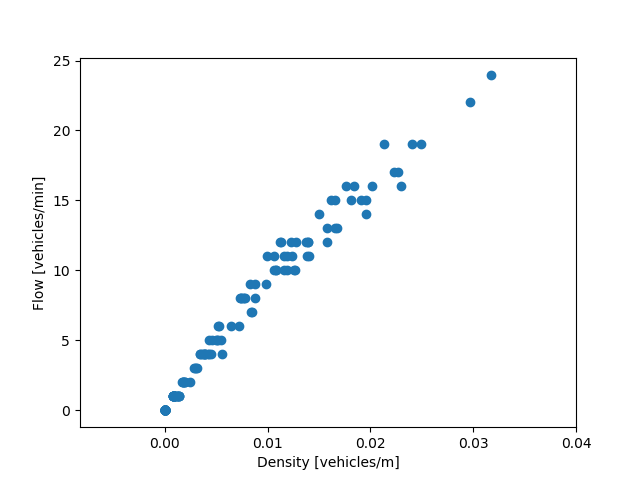
\includegraphics[width=0.45\textwidth]{graphs/Bulevardi_6_flw_dns.png}
    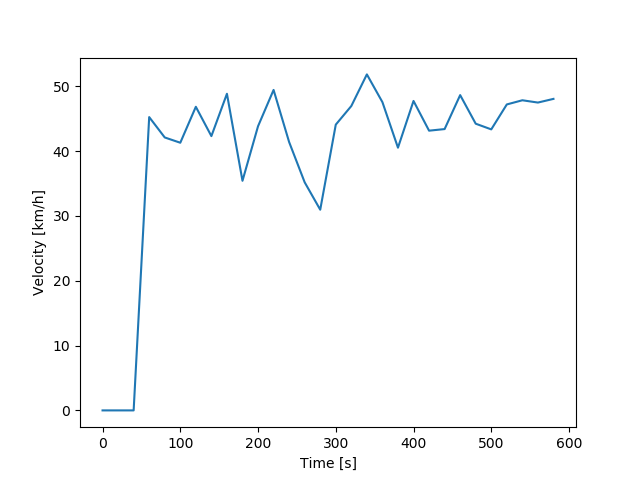
\includegraphics[width=0.45\textwidth]{graphs/Bulevardi_6_spd_time_6.png}
    \caption{Flow-density and velocity time series diagrams for Bulevardi, measurement point 6.}
\end{figure}
\begin{figure}[ht!]
    \centering
    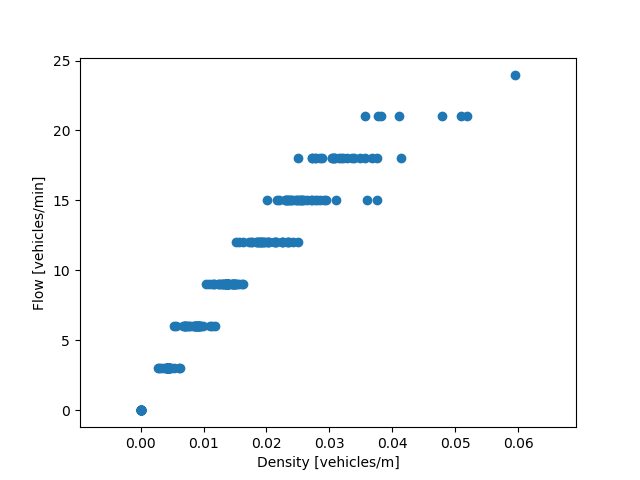
\includegraphics[width=0.45\textwidth]{graphs/Eerikinkatu_1_flw_dns.png}
    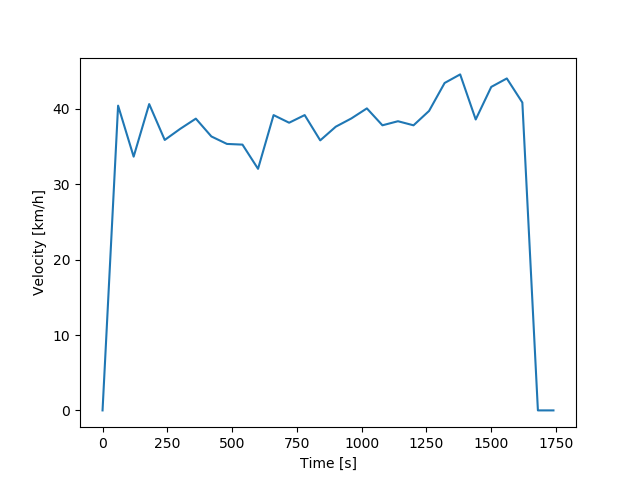
\includegraphics[width=0.45\textwidth]{graphs/Eerikinkatu_1_spd_time_6.png}
    \caption{Flow-density and velocity time series diagrams for Eerikinkatu, measurement point 1.}
\end{figure}
\begin{figure}[ht!]
    \centering
    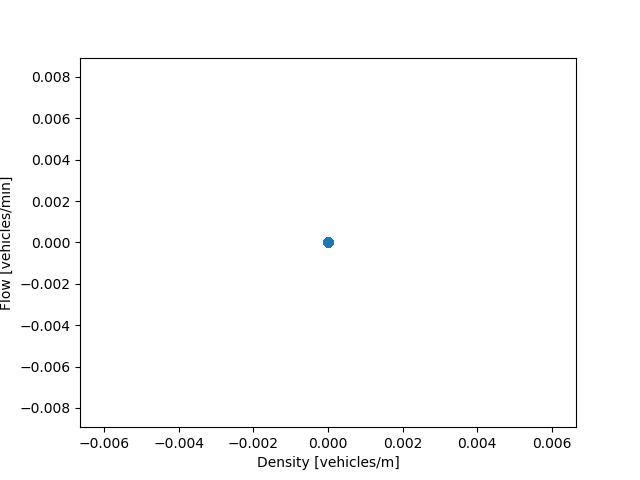
\includegraphics[width=0.45\textwidth]{graphs/Eerikinkatu_2_flw_dns.png}
    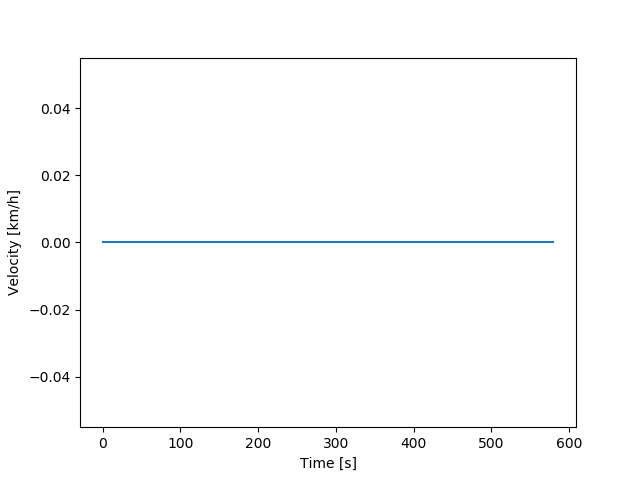
\includegraphics[width=0.45\textwidth]{graphs/Eerikinkatu_2_spd_time_6.png}
    \caption{Flow-density and velocity time series diagrams for Eerikinkatu, measurement point 2.}
\end{figure}

\clearpage
\begin{figure}[ht!]
    \centering
    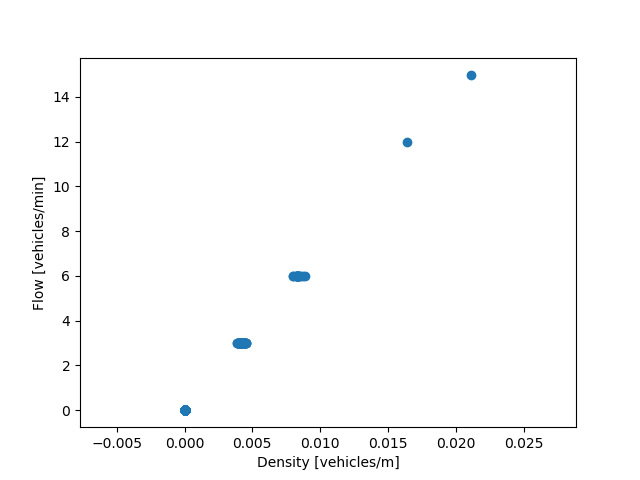
\includegraphics[width=0.45\textwidth]{graphs/Eerikinkatu_3_flw_dns.png}
    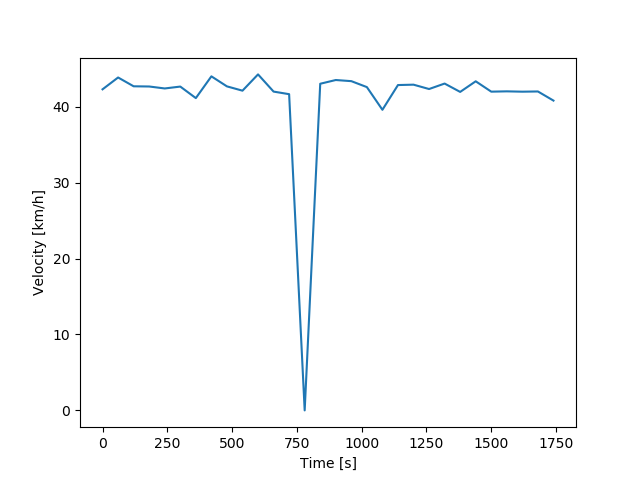
\includegraphics[width=0.45\textwidth]{graphs/Eerikinkatu_3_spd_time_6.png}
    \caption{Flow-density and velocity time series diagrams for Eerikinkatu, measurement point 3.}
\end{figure}
\begin{figure}[ht!]
    \centering
    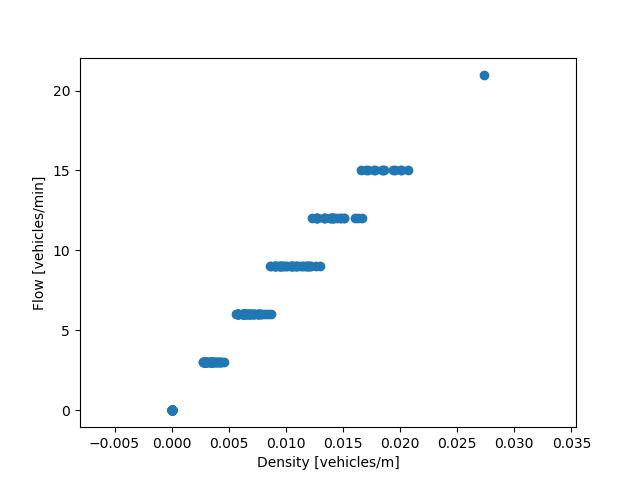
\includegraphics[width=0.45\textwidth]{graphs/Eerikinkatu_4_flw_dns.png}
    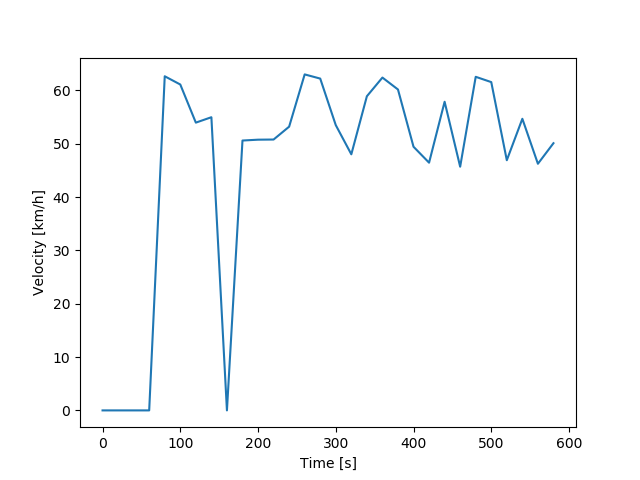
\includegraphics[width=0.45\textwidth]{graphs/Eerikinkatu_4_spd_time_6.png}
    \caption{Flow-density and velocity time series diagrams for Eerikinkatu, measurement point 4.}
\end{figure}
\begin{figure}[ht!]
    \centering
    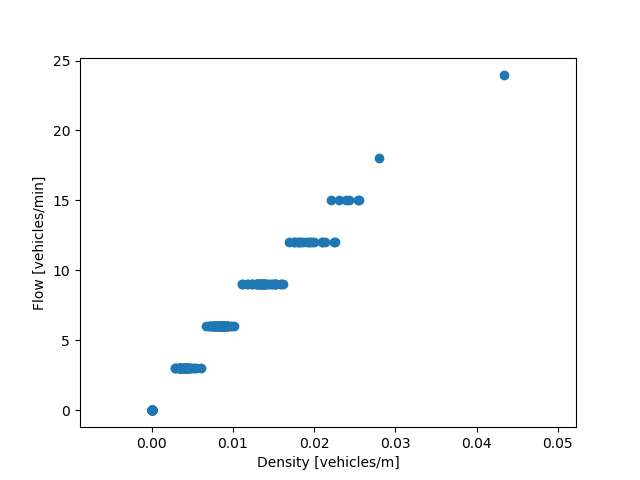
\includegraphics[width=0.45\textwidth]{graphs/Eerikinkatu_5_flw_dns.png}
    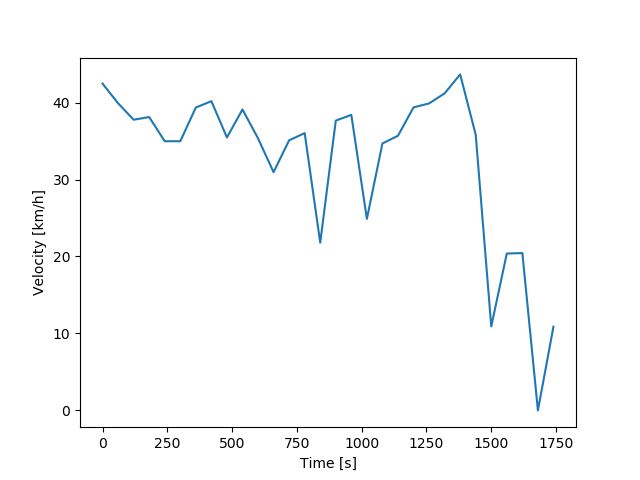
\includegraphics[width=0.45\textwidth]{graphs/Eerikinkatu_5_spd_time_6.png}
    \caption{Flow-density and velocity time series diagrams for Eerikinkatu, measurement point 5.}
\end{figure}

\clearpage
\begin{figure}[ht!]
    \centering
    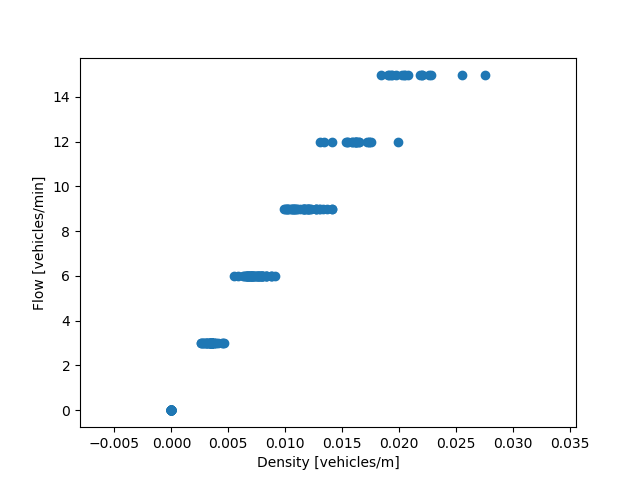
\includegraphics[width=0.45\textwidth]{graphs/Eerikinkatu_6_flw_dns.png}
    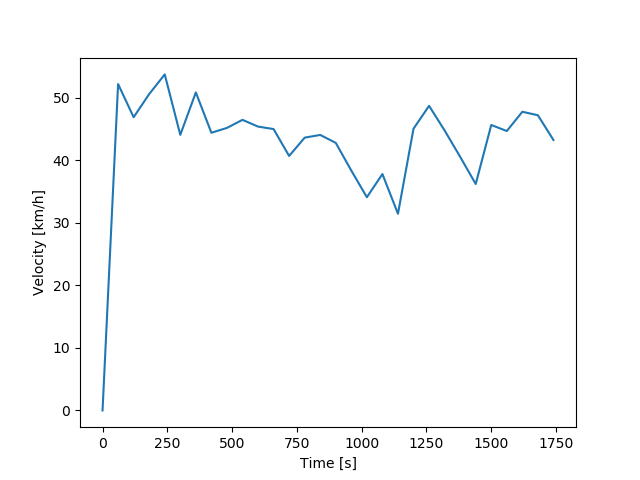
\includegraphics[width=0.45\textwidth]{graphs/Eerikinkatu_6_spd_time_6.png}
    \caption{Flow-density and velocity time series diagrams for Eerikinkatu, measurement point 6.}
\end{figure}
\begin{figure}[ht!]
    \centering
    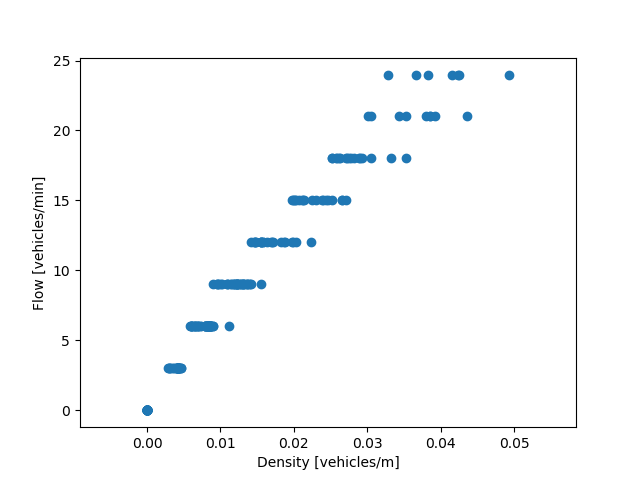
\includegraphics[width=0.45\textwidth]{graphs/Erottaja_1_flw_dns.png}
    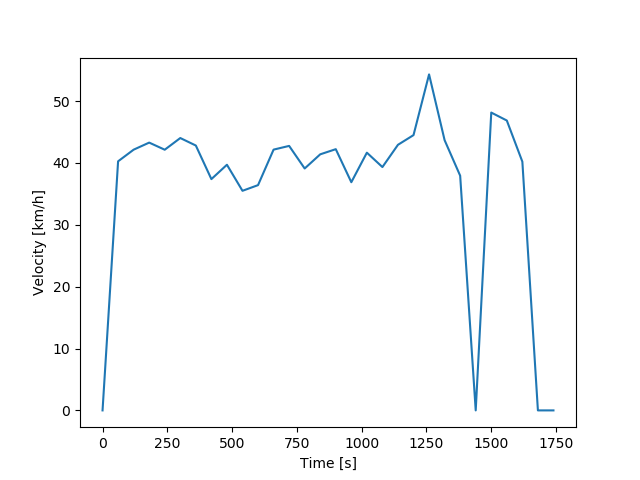
\includegraphics[width=0.45\textwidth]{graphs/Erottaja_1_spd_time_6.png}
    \caption{Flow-density and velocity time series diagrams for Erottaja, measurement point 1.}
\end{figure}
\begin{figure}[ht!]
    \centering
    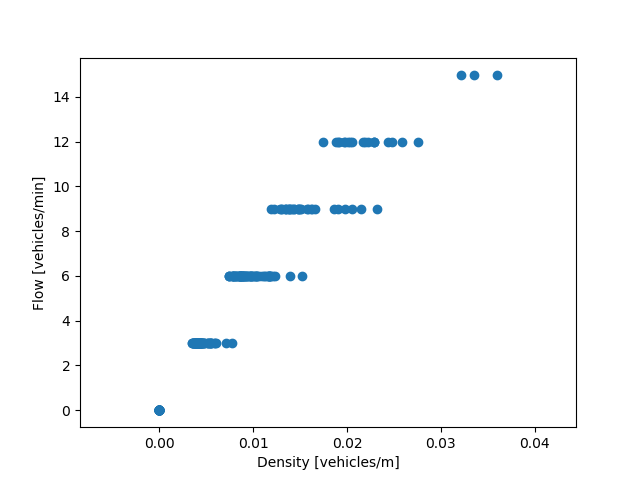
\includegraphics[width=0.45\textwidth]{graphs/Erottaja_2_flw_dns.png}
    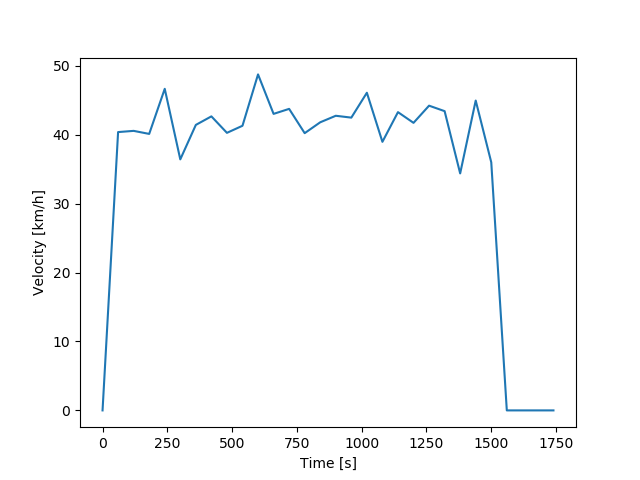
\includegraphics[width=0.45\textwidth]{graphs/Erottaja_2_spd_time_6.png}
    \caption{Flow-density and velocity time series diagrams for Erottaja, measurement point 2.}
\end{figure}

\clearpage
\begin{figure}[ht!]
    \centering
    \includegraphics[width=0.45\textwidth]{graphs/Etelaesplanadi_1_flw_dns.png}
    \includegraphics[width=0.45\textwidth]{graphs/Etelaesplanadi_1_spd_time_6.png}
    \caption{Flow-density and velocity time series diagrams for Etelaesplanadi, measurement point 1.}
\end{figure}
\begin{figure}[ht!]
    \centering
    \includegraphics[width=0.45\textwidth]{graphs/Hietalahdenranta_1_flw_dns.png}
    \includegraphics[width=0.45\textwidth]{graphs/Hietalahdenranta_1_spd_time_6.png}
    \caption{Flow-density and velocity time series diagrams for Hietalahdenranta, measurement point 1.}
\end{figure}
\begin{figure}[ht!]
    \centering
    \includegraphics[width=0.45\textwidth]{graphs/Hietalahdenranta_2_flw_dns.png}
    \includegraphics[width=0.45\textwidth]{graphs/Hietalahdenranta_2_spd_time_6.png}
    \caption{Flow-density and velocity time series diagrams for Hietalahdenranta, measurement point 2.}
\end{figure}

\clearpage
\begin{figure}[ht!]
    \centering
    \includegraphics[width=0.45\textwidth]{graphs/Jatkasaarenlaituri_1_flw_dns.png}
    \includegraphics[width=0.45\textwidth]{graphs/Jatkasaarenlaituri_1_spd_time_6.png}
    \caption{Flow-density and velocity time series diagrams for Jatkasaarenlaituri, measurement point 1.}
\end{figure}
\begin{figure}[ht!]
    \centering
    \includegraphics[width=0.45\textwidth]{graphs/Jatkasaarenlaituri_2_flw_dns.png}
    \includegraphics[width=0.45\textwidth]{graphs/Jatkasaarenlaituri_2_spd_time_6.png}
    \caption{Flow-density and velocity time series diagrams for Jatkasaarenlaituri, measurement point 2.}
\end{figure}
\begin{figure}[ht!]
    \centering
    \includegraphics[width=0.45\textwidth]{graphs/Kalevankatu_1_flw_dns.png}
    \includegraphics[width=0.45\textwidth]{graphs/Kalevankatu_1_spd_time_6.png}
    \caption{Flow-density and velocity time series diagrams for Kalevankatu, measurement point 1.}
\end{figure}

\clearpage
\begin{figure}[ht!]
    \centering
    \includegraphics[width=0.45\textwidth]{graphs/Kalevankatu_2_flw_dns.png}
    \includegraphics[width=0.45\textwidth]{graphs/Kalevankatu_2_spd_time_6.png}
    \caption{Flow-density and velocity time series diagrams for Kalevankatu, measurement point 2.}
\end{figure}
\begin{figure}[ht!]
    \centering
    \includegraphics[width=0.45\textwidth]{graphs/Kalevankatu_3_flw_dns.png}
    \includegraphics[width=0.45\textwidth]{graphs/Kalevankatu_3_spd_time_6.png}
    \caption{Flow-density and velocity time series diagrams for Kalevankatu, measurement point 3.}
\end{figure}
\begin{figure}[ht!]
    \centering
    \includegraphics[width=0.45\textwidth]{graphs/Kalevankatu_4_flw_dns.png}
    \includegraphics[width=0.45\textwidth]{graphs/Kalevankatu_4_spd_time_6.png}
    \caption{Flow-density and velocity time series diagrams for Kalevankatu, measurement point 4.}
\end{figure}

\clearpage
\begin{figure}[ht!]
    \centering
    \includegraphics[width=0.45\textwidth]{graphs/Korkeavuorenkatu_1_flw_dns.png}
    \includegraphics[width=0.45\textwidth]{graphs/Korkeavuorenkatu_1_spd_time_6.png}
    \caption{Flow-density and velocity time series diagrams for Korkeavuorenkatu, measurement point 1.}
\end{figure}
\begin{figure}[ht!]
    \centering
    \includegraphics[width=0.45\textwidth]{graphs/Korkeavuorenkatu_2_flw_dns.png}
    \includegraphics[width=0.45\textwidth]{graphs/Korkeavuorenkatu_2_spd_time_6.png}
    \caption{Flow-density and velocity time series diagrams for Korkeavuorenkatu, measurement point 2.}
\end{figure}
\begin{figure}[ht!]
    \centering
    \includegraphics[width=0.45\textwidth]{graphs/Korkeavuorenkatu_3_flw_dns.png}
    \includegraphics[width=0.45\textwidth]{graphs/Korkeavuorenkatu_3_spd_time_6.png}
    \caption{Flow-density and velocity time series diagrams for Korkeavuorenkatu, measurement point 3.}
\end{figure}

\clearpage
\begin{figure}[ht!]
    \centering
    \includegraphics[width=0.45\textwidth]{graphs/Korkeavuorenkatu_4_flw_dns.png}
    \includegraphics[width=0.45\textwidth]{graphs/Korkeavuorenkatu_4_spd_time_6.png}
    \caption{Flow-density and velocity time series diagrams for Korkeavuorenkatu, measurement point 4.}
\end{figure}
\begin{figure}[ht!]
    \centering
    \includegraphics[width=0.45\textwidth]{graphs/Lansivayla_1_flw_dns.png}
    \includegraphics[width=0.45\textwidth]{graphs/Lansivayla_1_spd_time_6.png}
    \caption{Flow-density and velocity time series diagrams for Lansivayla, measurement point 1.}
\end{figure}
\begin{figure}[ht!]
    \centering
    \includegraphics[width=0.45\textwidth]{graphs/Lansivayla_2_flw_dns.png}
    \includegraphics[width=0.45\textwidth]{graphs/Lansivayla_2_spd_time_6.png}
    \caption{Flow-density and velocity time series diagrams for Lansivayla, measurement point 2.}
\end{figure}

\clearpage
\begin{figure}[ht!]
    \centering
    \includegraphics[width=0.45\textwidth]{graphs/Lonnrotinkatu_1_flw_dns.png}
    \includegraphics[width=0.45\textwidth]{graphs/Lonnrotinkatu_1_spd_time_6.png}
    \caption{Flow-density and velocity time series diagrams for Lönnrotinkatu, measurement point 1.}
\end{figure}
\begin{figure}[ht!]
    \centering
    \includegraphics[width=0.45\textwidth]{graphs/Lonnrotinkatu_2_flw_dns.png}
    \includegraphics[width=0.45\textwidth]{graphs/Lonnrotinkatu_2_spd_time_6.png}
    \caption{Flow-density and velocity time series diagrams for Lönnrotinkatu, measurement point 2.}
\end{figure}
\begin{figure}[ht!]
    \centering
    \includegraphics[width=0.45\textwidth]{graphs/Lonnrotinkatu_3_flw_dns.png}
    \includegraphics[width=0.45\textwidth]{graphs/Lonnrotinkatu_3_spd_time_6.png}
    \caption{Flow-density and velocity time series diagrams for Lönnrotinkatu, measurement point 3.}
\end{figure}

\clearpage
\begin{figure}[ht!]
    \centering
    \includegraphics[width=0.45\textwidth]{graphs/Lonnrotinkatu_4_flw_dns.png}
    \includegraphics[width=0.45\textwidth]{graphs/Lonnrotinkatu_4_spd_time_6.png}
    \caption{Flow-density and velocity time series diagrams for Lönnrotinkatu, measurement point 4.}
\end{figure}
\begin{figure}[ht!]
    \centering
    \includegraphics[width=0.45\textwidth]{graphs/Malminrinne_1_flw_dns.png}
    \includegraphics[width=0.45\textwidth]{graphs/Malminrinne_1_spd_time_6.png}
    \caption{Flow-density and velocity time series diagrams for Malminrinne, measurement point 1.}
\end{figure}
\begin{figure}[ht!]
    \centering
    \includegraphics[width=0.45\textwidth]{graphs/Malminrinne_2_flw_dns.png}
    \includegraphics[width=0.45\textwidth]{graphs/Malminrinne_2_spd_time_6.png}
    \caption{Flow-density and velocity time series diagrams for Malminrinne, measurement point 2.}
\end{figure}

\clearpage
\begin{figure}[ht!]
    \centering
    \includegraphics[width=0.45\textwidth]{graphs/Mannerheimintie_1_flw_dns.png}
    \includegraphics[width=0.45\textwidth]{graphs/Mannerheimintie_1_spd_time_6.png}
    \caption{Flow-density and velocity time series diagrams for Mannerheimintie, measurement point 1.}
\end{figure}
\begin{figure}[ht!]
    \centering
    \includegraphics[width=0.45\textwidth]{graphs/Mannerheimintie_2_flw_dns.png}
    \includegraphics[width=0.45\textwidth]{graphs/Mannerheimintie_2_spd_time_6.png}
    \caption{Flow-density and velocity time series diagrams for Mannerheimintie, measurement point 2.}
\end{figure}
\begin{figure}[ht!]
    \centering
    \includegraphics[width=0.45\textwidth]{graphs/Mannerheimintie_3_flw_dns.png}
    \includegraphics[width=0.45\textwidth]{graphs/Mannerheimintie_3_spd_time_6.png}
    \caption{Flow-density and velocity time series diagrams for Mannerheimintie, measurement point 3.}
\end{figure}

\clearpage
\begin{figure}[ht!]
    \centering
    \includegraphics[width=0.45\textwidth]{graphs/Mannerheimintie_4_flw_dns.png}
    \includegraphics[width=0.45\textwidth]{graphs/Mannerheimintie_4_spd_time_6.png}
    \caption{Flow-density and velocity time series diagrams for Mannerheimintie, measurement point 4.}
\end{figure}
\begin{figure}[ht!]
    \centering
    \includegraphics[width=0.45\textwidth]{graphs/Mechelininkatu_1_flw_dns.png}
    \includegraphics[width=0.45\textwidth]{graphs/Mechelininkatu_1_spd_time_6.png}
    \caption{Flow-density and velocity time series diagrams for Mechelininkatu, measurement point 1.}
\end{figure}
\begin{figure}[ht!]
    \centering
    \includegraphics[width=0.45\textwidth]{graphs/Mechelininkatu_2_flw_dns.png}
    \includegraphics[width=0.45\textwidth]{graphs/Mechelininkatu_2_spd_time_6.png}
    \caption{Flow-density and velocity time series diagrams for Mechelininkatu, measurement point 2.}
\end{figure}

\clearpage
\begin{figure}[ht!]
    \centering
    \includegraphics[width=0.45\textwidth]{graphs/Mechelininkatu_3_flw_dns.png}
    \includegraphics[width=0.45\textwidth]{graphs/Mechelininkatu_3_spd_time_6.png}
    \caption{Flow-density and velocity time series diagrams for Mechelininkatu, measurement point 3.}
\end{figure}
\begin{figure}[ht!]
    \centering
    \includegraphics[width=0.45\textwidth]{graphs/Mechelininkatu_4_flw_dns.png}
    \includegraphics[width=0.45\textwidth]{graphs/Mechelininkatu_4_spd_time_6.png}
    \caption{Flow-density and velocity time series diagrams for Mechelininkatu, measurement point 4.}
\end{figure}
\begin{figure}[ht!]
    \centering
    \includegraphics[width=0.45\textwidth]{graphs/Pohjoisesplanadi_1_flw_dns.png}
    \includegraphics[width=0.45\textwidth]{graphs/Pohjoisesplanadi_1_spd_time_6.png}
    \caption{Flow-density and velocity time series diagrams for Pohjoisesplanadi, measurement point 1.}
\end{figure}

\clearpage
\begin{figure}[ht!]
    \centering
    \includegraphics[width=0.45\textwidth]{graphs/Porkkalankatu_1_flw_dns.png}
    \includegraphics[width=0.45\textwidth]{graphs/Porkkalankatu_1_spd_time_6.png}
    \caption{Flow-density and velocity time series diagrams for Porkkalankatu, measurement point 1.}
\end{figure}
\begin{figure}[ht!]
    \centering
    \includegraphics[width=0.45\textwidth]{graphs/Porkkalankatu_2_flw_dns.png}
    \includegraphics[width=0.45\textwidth]{graphs/Porkkalankatu_2_spd_time_6.png}
    \caption{Flow-density and velocity time series diagrams for Porkkalankatu, measurement point 2.}
\end{figure}
\begin{figure}[ht!]
    \centering
    \includegraphics[width=0.45\textwidth]{graphs/Punavuorenkatu_1_flw_dns.png}
    \includegraphics[width=0.45\textwidth]{graphs/Punavuorenkatu_1_spd_time_6.png}
    \caption{Flow-density and velocity time series diagrams for Punavuorenkatu, measurement point 1.}
\end{figure}

\clearpage
\begin{figure}[ht!]
    \centering
    \includegraphics[width=0.45\textwidth]{graphs/Punavuorenkatu_2_flw_dns.png}
    \includegraphics[width=0.45\textwidth]{graphs/Punavuorenkatu_2_spd_time_6.png}
    \caption{Flow-density and velocity time series diagrams for Punavuorenkatu, measurement point 2.}
\end{figure}
\begin{figure}[ht!]
    \centering
    \includegraphics[width=0.45\textwidth]{graphs/Ruoholahdenkatu_1_flw_dns.png}
    \includegraphics[width=0.45\textwidth]{graphs/Ruoholahdenkatu_1_spd_time_6.png}
    \caption{ Flow-density and velocity time series diagrams for Ruoholahdenkatu, measurement point 1. }
\end{figure}
\begin{figure}[ht!]
    \centering
    \includegraphics[width=0.45\textwidth]{graphs/Uudenmaankatu_1_flw_dns.png}
    \includegraphics[width=0.45\textwidth]{graphs/Uudenmaankatu_1_spd_time_6.png}
    \caption{Flow-density and velocity time series diagrams for Uudenmaankatu, measurement point 1.}
\end{figure}

\clearpage
\begin{figure}[ht!]
    \centering
    \includegraphics[width=0.45\textwidth]{graphs/Uudenmaankatu_2_flw_dns.png}
    \includegraphics[width=0.45\textwidth]{graphs/Uudenmaankatu_2_spd_time_6.png}
    \caption{Flow-density and velocity time series diagrams for Uudenmaankatu, measurement point 2.}
\end{figure}
\begin{figure}[ht!]
    \centering
    \includegraphics[width=0.45\textwidth]{graphs/Yrjonkatu_1_flw_dns.png}
    \includegraphics[width=0.45\textwidth]{graphs/Yrjonkatu_1_spd_time_6.png}
    \caption{Flow-density and velocity time series diagrams for Yrjönkatu, measurement point 1.}
\end{figure}
\begin{figure}[ht!]
    \centering
    \includegraphics[width=0.45\textwidth]{graphs/Yrjonkatu_2_flw_dns.png}
    \includegraphics[width=0.45\textwidth]{graphs/Yrjonkatu_2_spd_time_6.png}
    \caption{Flow-density and velocity time series diagrams for Yrjönkatu, measurement point 2.}
\end{figure}

\clearpage

\end{document}
